\chapter{Results} % Main appendix title
\label{Appendix-results} % For referencing this appendix elsewhere, use 

%%%%%%%%%%%%%%%%%%%%%%%%%%%%%%%%%%%%%%%%%%%%%%%%%%%%%%%%%%%%%%%%%%%%%%%%%%%%%
% RUN XX - TEMPLATE - experiment log template
%%%%%%%%%%%%%%%%%%%%%%%%%%%%%%%%%%%%%%%%%%%%%%%%%%%%%%%%%%%%%%%%%%%%%%%%%%%%%
%\subsection{Run XX -  }
%\label{app_res:XX}
%\begin{verbatim}
%Commit:
%Model: 
%Outputs: 
%Dataset: 
%Command:
%Environment: 
%Comment: 
%\end{verbatim}

%%%%%%%%%%%%%%%%%%%%%%%%%%%%%%%%%%%%%%%%%%%%%%%%%%%%%%%%%%%%%%%%%%%%%%%%%%%%%
% RUN XX - TEMPLATE - experiment log template
%%%%%%%%%%%%%%%%%%%%%%%%%%%%%%%%%%%%%%%%%%%%%%%%%%%%%%%%%%%%%%%%%%%%%%%%%%%%%

\subsection{Run 01 - RealSense Viewer}

\label{app_res:01}

Started RealSense Viewer (v2.45.0): 
\begin{verbatim}
$ realsense-viewer    
\end{verbatim}
Updated camera firmware to version 5.12.13.50 from 05.12.11.00.
Screen capture uploaded to \Url{https://youtu.be/eltQ_hvpcFs}
% Kazam 
% Windows key + CTRL + R = Start recording.
% Windows key + CTRL + P = Pause recording, press again to resume.
% Windows key + CTRL + F = Finish recording.
% Windows key + CTRL + Q = Quit recording.

\subsection{Run 02 - Viewing Realsense Viewer point cloud output}
\label{app_res:01}

We output 3 files: output\_meshing\_no\_normals.ply, output\_meshing\_normals.ply and output\_no\_meshing\_no\_normals.ply. We then visualise with Open3D:
\begin{verbatim}
# from open3d import *    
import open3d as o3d

def main():
    cloud = o3d.io.read_point_cloud("output_meshing_normals.ply") # Read the point cloud
    o3d.visualization.draw_geometries([cloud]) # Visualize the point cloud     

if __name__ == "__main__":
    main()
\end{verbatim}
The output provides a mean of performing qualitative analysis on cleargrasp depth completion.
\begin{figure}[h!]
\centering
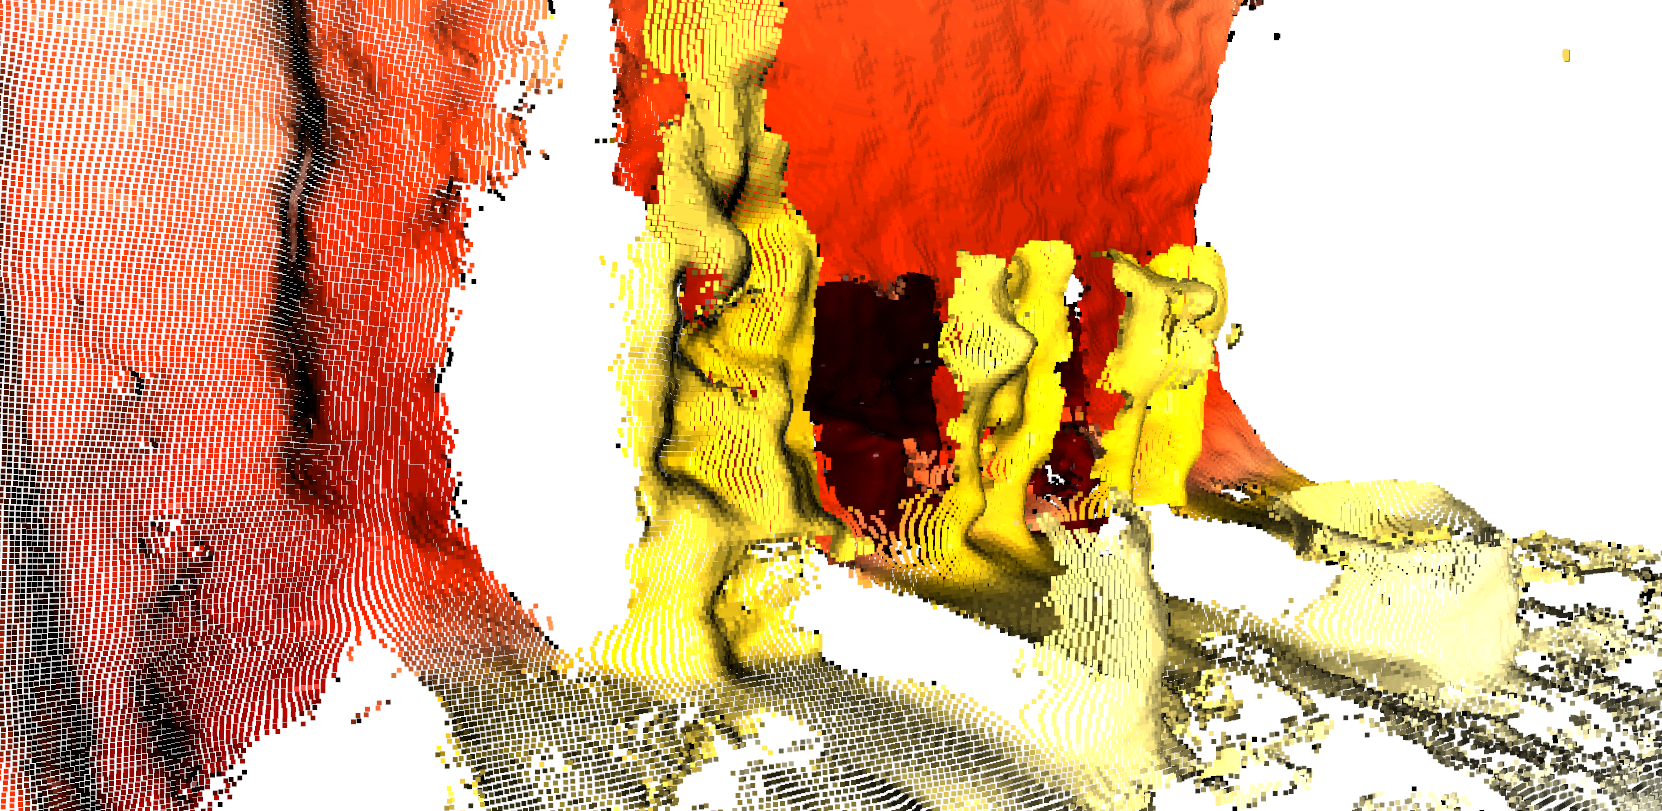
\includegraphics[width=\textwidth]{Figures/OpenCV-point-cloud-import-2.png}
\caption{RealSense Viewer D415 point cloud output rendered with OpenCV}
\label{fig:realsenseOutputForReport}
\end{figure}




